\documentclass{patmorin}
\usepackage{pat,graphicx}

\newcommand{\VG}{\mathit{VG}}
\newcommand{\VSP}{\mathit{VSP}}

\title{\MakeUppercase{Covering Visibility Polygons with Triangles:\newline
       Algorithms and Applications}}
\author{Joachim Gudmundsson\thanks{\affil{NICTA},
\email{joachim.gudmundsson@nicta.com.au}}\, 
       and Pat Morin\thanks{\affil{Carleton University},
\email{morin@scs.carleton.ca}}}

\begin{document}
\maketitle
\begin{abstract}
Let $S$ be a set of $n$ disjoint line segments in $\R^2$ and let $s$
be an element of $S$.  An example due to So and So shows that the
subset, $V_S(s)$, of $\R^2$ weakly visible from $s$ can have complexity
$\Omega(n^4)$.  In the current paper we show that $V_S(s)$ can always
be covered by a set $C_S(s)$ of $O(n^2)$ triangles.  More generally,
we show that the expected number of triangles needed to cover $V(S,s)$
for a random element $s\in S$ is $O(n)$.

Storing the triangles $C_S(s)$ in a partition (Welzl XX, Matou\v{s}ek YY)
tree yields an efficient data structure for testing if a query point is
contained in $V_S(s)$. Using random sampling, this yields an efficient
data structure for (additively) approximating the number of elements of
$S$ that are at least partially visible from a query point.  Furthermore,
the structure of the triangles used in these coverings is such that,
storing the $O(m)$ triangles of $\bigcup_{s\in S} C_S(s)$ in a partition
tree yields an efficient data structure for finding a 3-approximation
of the number of segments of $S$ partially visible from a query point.
Here $m\le 2n^2-n$ is the number of edges in the visibility graph of $S$.
\end{abstract}

\section{Introduction}

The elements of $S$ are closed line segments and are disjoint in the sense
that there are not two elements $s_1,s_2\in S$, with $s_1\neq s_2$, such
that the interior of $s_1$ and the interior of $s_2$ have a point in
common.

Two points $p,q\in\R^2$ are \emph{visible} if the open line segment $pq$
does not intersect any element of $S$.  A segment $s\in S$ is (weakly)
\emph{visible} from a point $p$ if there exists a point $q\in S$ such that
$p$ and $q$ are visible.

For a point $p\in\R^2$, the \emph{visibility region} or \emph{visibility
polygon} of $p$ (with respect to $S$) is defined as
\[
   V_S(p)=\{q\in\R^2:\mbox{$p$ and $q$ are visible}\}
\]
For a segment $s\in S$, the \emph{visibility region} of $s$ (with respect
to $S$)
\[
   V_S(s)=\bigcup_{p\in s} V_S(p) \enspace 
\]
is the set of points in $\R^2$ that are visible from some point on $s$.

The \emph{visibility graph} $\VG(S)$ is a graph whose vertices are the $2n$
endpoints of the elements in $S$ and in which the edge $pq$ exists if and
only if the open line segment with endpoints $p$ and $q$ does not intersect
any (closed) segment in $S$.  It is well-known that the number of edges in
$\VG(S)$ is in $\Omega(n)\cap O(n^2)$.

Consider extending each edge of the visibility graph in both directions
until it intersects an element of $S$ or goes off to infinity (see
\figref{vsp}). The union of these extended visibility graph edges and
segments in $S$ form a 1-dimensional set whose removal disconnects $\R^2$
into a set of 2-dimensional regions.  This set of 2-d regions is known as
the \emph{visibility space partition}, $\VSP(S)$ of $S$.  The regions of
$\VSP(S)$ are important because any region $R\in\VSP(S)$ does not intersect
$V_S(s)$ for any element $s\in S$;  for any $p,q\in R$ the set of segments
of $S$ visible from $p$ is equal to the set of segments of $S$ visible from
$q$.  

Note that $\VSP(S)$ is defined by $O(n^2)$ line segments, lines, and rays
so that it has complexity $O(n^4)$.  The example in \figref{quartic} shows
an example where this quartic complexity is achieved.

\section{Covering $V_S(s)$}

In this section we give an algorithm for covering $V_S(s)$ with triangles.
The number of triangles used in the covering is bounded by $O(n+m_s)$ where
$m_s$ is the number of vertices of $\VSP(S)$ that are incident to $s$.

Assume, without loss of generality, that $s$ is horizontal.  We will show
how to cover the portion of $V_S(s)$ in the halfplane bounded from below by
the supporting line of $s$.  The complementary part of $V_S(s)$ can be
covered with a symmetric algorithm.

The algorithm works by sweeping a point $p$ from left to right across the
segment $s$.  Events in this sweep occur at the vertices
$p_1,\ldots,p_{m_s}$ of $V_S(s)$
incident on $s$, in their left to right order along $p$.  Initially $p=p_1$ is set to the left endpoint of $s$.  We
compute $V_S(p)$ and cover $V_S(p)$ with $O(n)$ triangles, each of which
has a vertex at $p$ in the obvious (see \figref{alg}.a).  Consider an edge or
ray $e$ of $V_S(p)$.  We say that $e$ is \emph{active} if the lower
endpoint of $e$ is incident to the right endpoint of a segment of $s$ (see
\figref{alg}).  Note that, as $p$ sweeps to the right, the active edges of
$p$ rotate about their lower endpoints, possibly exposing more of $\R^2$.

\begin{figure}
  \begin{center}
    \begin{tabular}{ccc}
      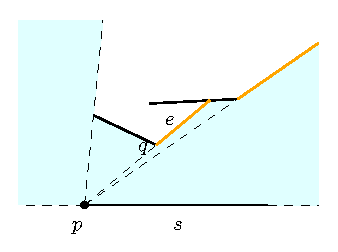
\includegraphics{alg-1} &
      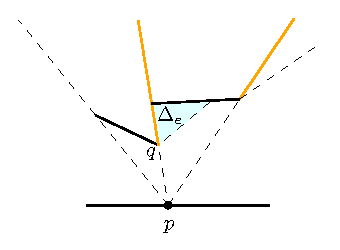
\includegraphics{alg-2} &
      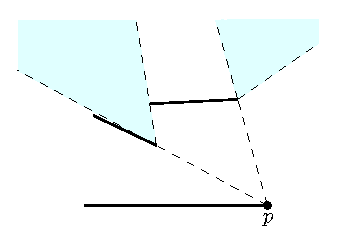
\includegraphics{alg-3} \\
      (a) & (b) & (c)
    \end{tabular}
  \end{center}
  \caption{The algorithm for covering $V_S(s)$ with triangles processing
           the events at (a)~$p_1$, (b)~$p_2$ and (c)~$p_3$.  
           Active edges are shown in orange and triangles in the covering
are shown at the time they are added to the covering.}
  \figlabel{alg}
\end{figure}

The crucial observation underlying the algorithm is the following:
$V_S(p_i) \setminus V_S(p_{i-1})$ can be covered by triangles, each of
which is incident to an active edge of $V_S(p_{i-1})$.

To see how this observation is used, consider advancing $p$ from $p_1$ to
$p_2$.  If $p_2$ is not defined by an active edge of $V_S(p)$ then we do
nothing.  Otherwise, consider the active edge $e$ that defines (and hence
is collinear with) $p_2$.  While travelling from $p_1$ to $p_2$, $p$ has
seen every point in a triangle $t$ with one vertex at the lower endpoint of
$e$ that is incident on one edge collinear with $p$ and another edge
collinear with $p_2$ (see \figref{alg}.b)}.  We add this triangle to the
cover $C_S(s)$.  At this point, another edge of $V_S(p)$ may become active.

In general, when advancing from $p_{i-1}$ to $p_{i}$ there are a number of
active edges.  Upon reaching $p_{i}$, $p$ becomes collinear with at most
one of these edges $e$, at which point we add a triangle to our cover.  This
triangle has one vertex at $e$ that is incident to two edges, one of which
is collinear with $p_{i}$ and the other that is collinear the point $p_j$,
$j < i$ at which edge $e$ became active.  At most one new

The algorithm terminates with $p$ reaches the right endpoint of $s$.  At
this time, all active edges are completed so that they form triangles.  The
union of all triangles created form a cover of $p$.







\end{document}
